%\subsection{Evaluación de los métodos}

%\subsubsection{Método utilizado para el calculo de la isoterma}

%Una vez obtenidas todas las temperaturas del sistema buscamos por cada ángulo del horno entre que dos puntos debería estar la temperatura buscada de la isoterma. Una vez localizados estos puntos suponemos que el crecimiento de la temperatura es lineal, lo cual no necesariamente es cierto pero si se toman puntos suficientemente cercanos el error es ínfimo, a partir de esta suposición podemos fácilmente plantear la ecuación de una recta que pasa por los dos puntos que conocemos y deducir de esto donde debería estar el punto que tiene la temperatura que nos interesa.

\subsection{Criterios de análisis para la isoterma}
 Para tener una referencia a partir de la cual decidir si el horno podía llegar a estar en peligro o no, decidimos utilizar tres criterios clásicos: el promedio, la mediana y el máximo, ya que cada uno presenta ciertos aspectos útiles.
 
  La media o promedio permite tener una idea general de los valores que tiene la isoterma, permitiendo darnos una idea básica de que tantos ángulos o con que tanta intensidad están superando el umbral, como desventaja presenta problemas al haber outliers en las mediciones de temperatura lo cual puede distorsionar la medición.
 
  La mediana permite solucionar el problema previo por su mayor robustez; medidas que estén fuera de lugar respecto de las que aparezcan por mayoría no afectarán el resultado final y se obtendrá una idea más clara del valor que se está teniendo mayormente mientras que los valores estén dentro de cierto rango acotado.
  
   El máximo permite ver picos que podrían pasar desapercibidos viendo únicamente la media o mediana pero como desventaja se pierden tendencias generales y los outliers lo afectan en gran medida.

Una vez escogidos estos criterios de análisis lo que hicimos fue, para una instancia de isoterma dada, ver si al calcular el promedio, mediana o máximo alguno supera cierto umbral escogido. De suceder esto entonces se dirá que el horno esta en peligro. Para elegir el umbral se aconseja basarse en casos previos de hornos de características similares que sufrieron daños, a partir de esto estudiar la isoterma en esos casos con los criterios establecidos previamente y deducir valores adecuados dentro de los cuales sea recomendable trabajar.

\subsection{Relación entre granularidad y precisión en el cálculo de la isoterma}
A través de una serie de experimentos buscamos estudiar que factores contribuyen a una mayor precisión en el cálculo de la posición de la isoterma. Logrando así una predicción más fiable del peligro en el que puede llegar a estar el horno y sin perder el tiempo con cálculos innecesarios.

Al realizar los experimentos nos interesamos en estudiar cómo la granularidad afectaba la precisión de la estimación de la isoterma, para así poder estar seguros si el horno estaba o no en peligro. Para hacer esto separamos los experimentos en dos, primero estudiamos qué pasaba cuando utilizábamos una mayor cantidad de ángulos y luego lo mismo para los radios.

En este documento presentamos las imágenes mas representativas de nuestra investigación pero para una mayor profundización se puede visitar el link de \ref{sec:links}) donde están todos nuestros experimentos sobre isotermas.


\subsubsection{Granularidad de los ángulos}

Antes de realizar los experimentos, nos planteamos nuestras hipótesis. Como al aumentar la cantidad de ángulos se podrán detectar mejor los cambios bruscos en la isoterma, esto permitirá ver con mayor claridad donde comienzan y donde acaban los picos mientras mejor sea la granularidad. En caso de utilizar una granularidad pobre se verán picos poco precisos o incluso gráficos de isotermas erróneos que fallan en detectar el pico, lo cual podría conllevar consecuencias muy graves al no advertir un posible peligro en el horno.

En este primer experimento se utiliza una instancia en la cual la temperatura en todos los ángulos externos es igual excepto en una pequeña zona donde aumenta. 
Si se piensa a $r_e$ y $r_i$ como listas, lo que hicimos para disminuir la granularidad fue empezar con dos listas de largo 50 y luego ir tomando primero los índices pares de cada lista, luego los índices múltiplos de 3, y así sucesivamente.

Este experimento puede pensarse como que disminuimos la cantidad de mediciones que tomamos de la temperatura dentro y fuera del horno, pero sin embargo manteniendo su equidistribución.


\begin{figure}[H]
\centering
\begin{minipage}{0.30\textwidth}
  \centering
    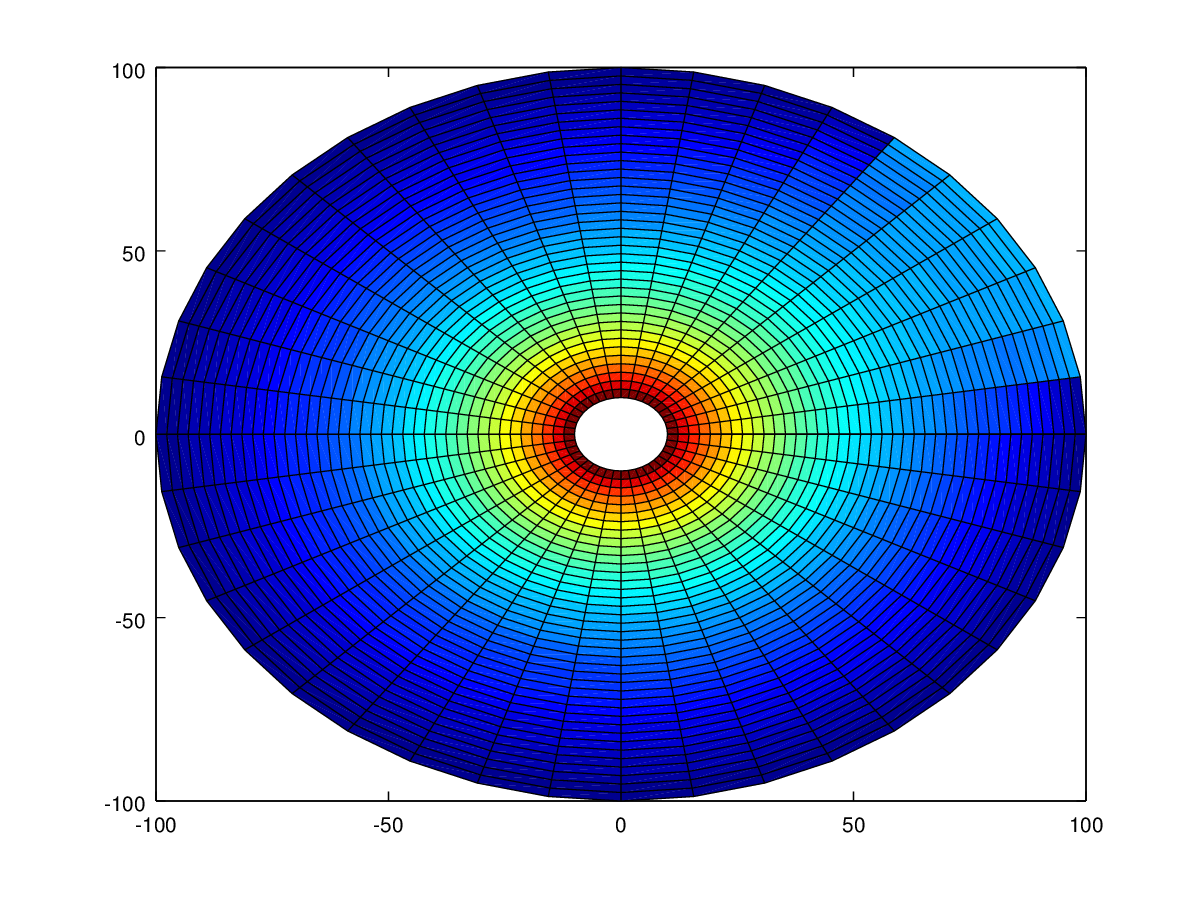
\includegraphics[width=1\textwidth]{imgs/comp_angulos/comp_angs_temp0.png}
  \caption{}
  \label{fig:comp_angs_temp0}
\end{minipage}%
\hspace{0.03\textwidth}
\begin{minipage}{0.30\textwidth}   
  \centering
    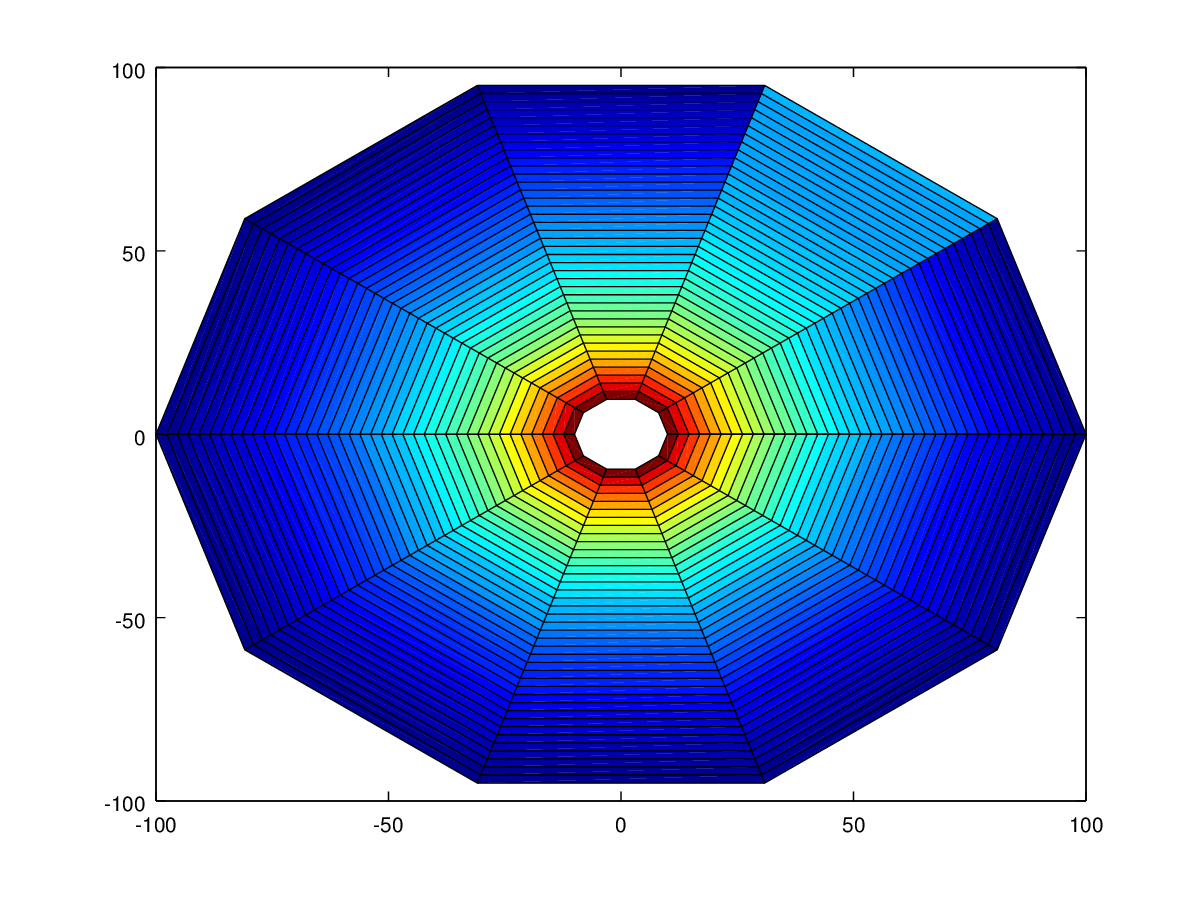
\includegraphics[width=1\textwidth]{imgs/comp_angulos/comp_angs_temp3.png} 
  \caption{}
  \label{fig:comp_angs_temp3}
\end{minipage}%
\hspace{0.03\textwidth}
\begin{minipage}{0.30\textwidth}   
  \centering
    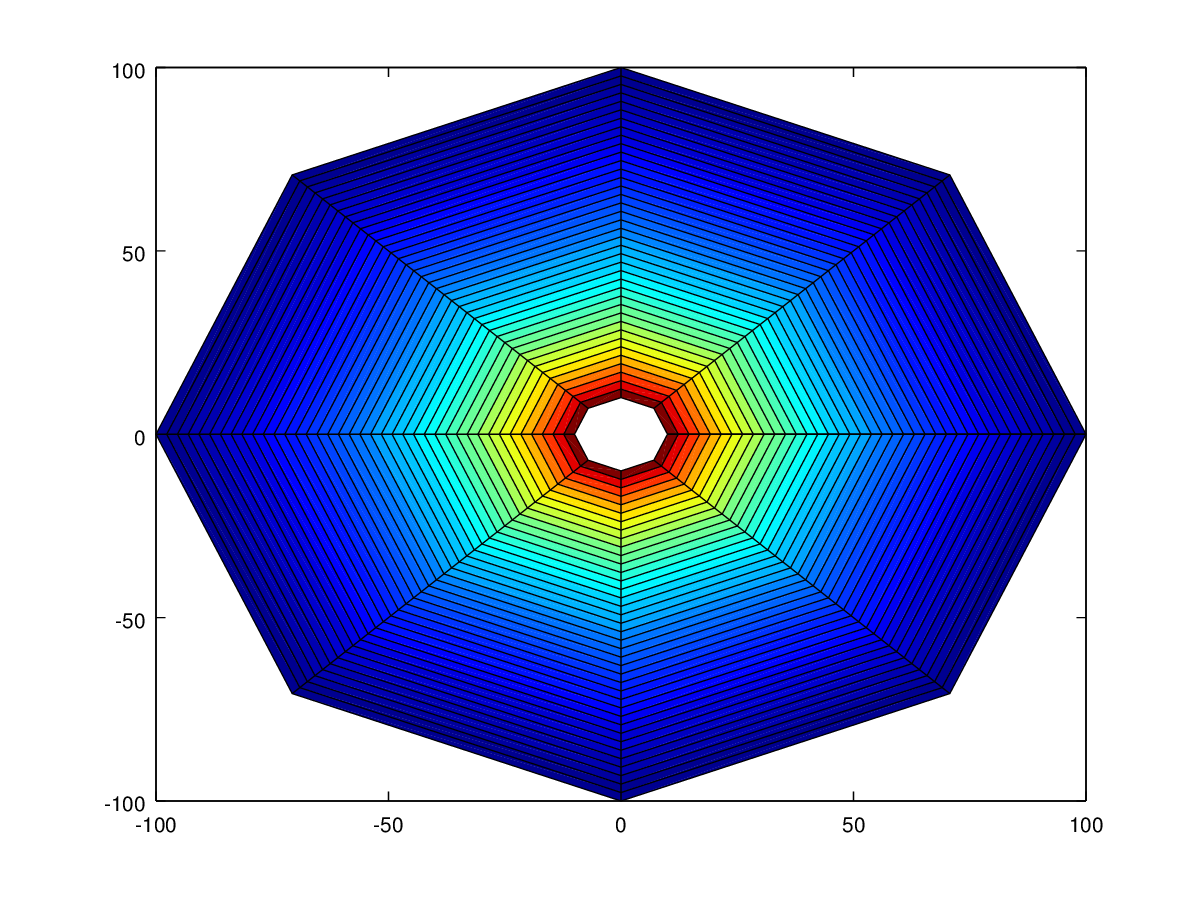
\includegraphics[width=1\textwidth]{imgs/comp_angulos/comp_angs_temp4.png} 
  \caption{}
  \label{fig:comp_angs_temp4}
\end{minipage}
\end{figure}


\begin{figure}[H]
\centering
\begin{minipage}{0.30\textwidth}
  \centering
    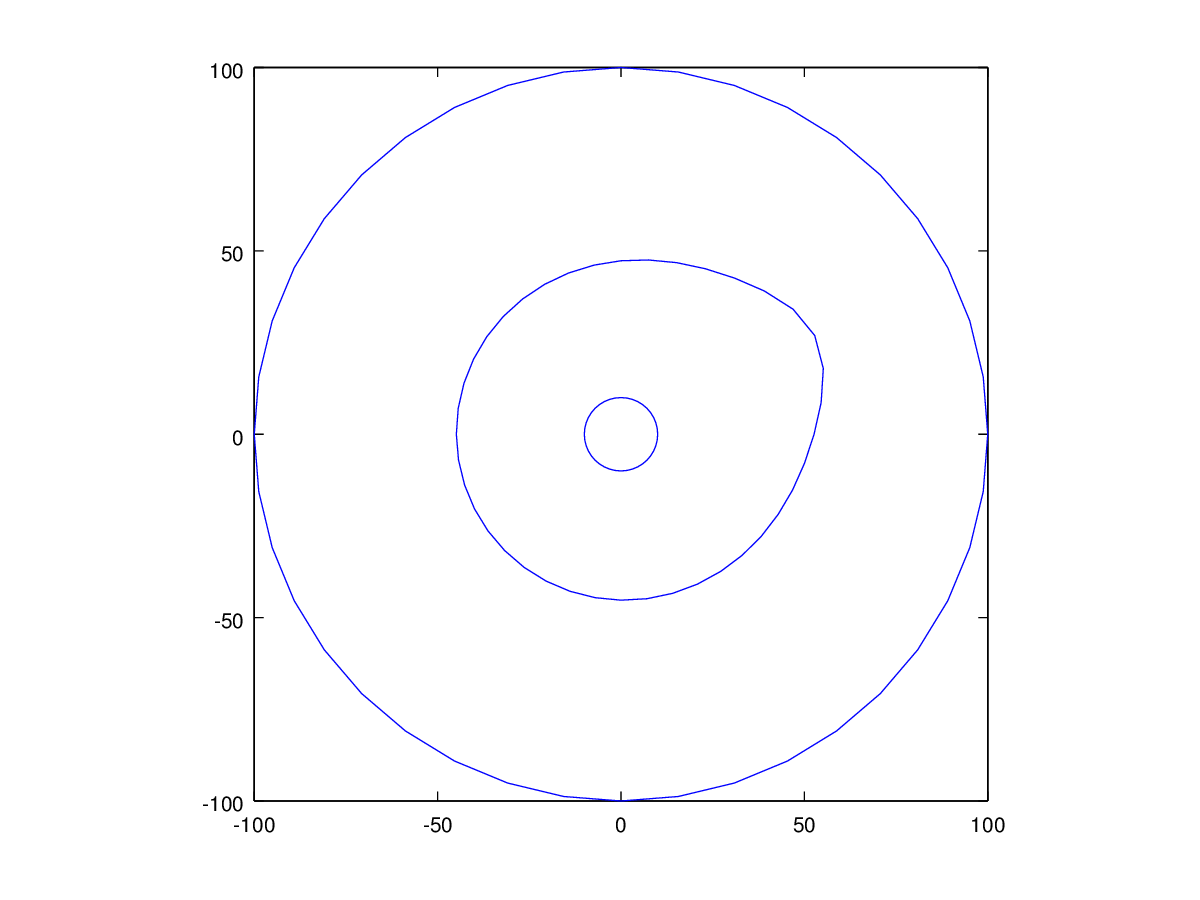
\includegraphics[width=1\textwidth]{imgs/comp_angulos/comp_angs_iso0.png}
  \caption{}
  \label{fig:comp_angs_iso0}
\end{minipage}%
\hspace{0.03\textwidth}
\begin{minipage}{0.30\textwidth}   
  \centering
    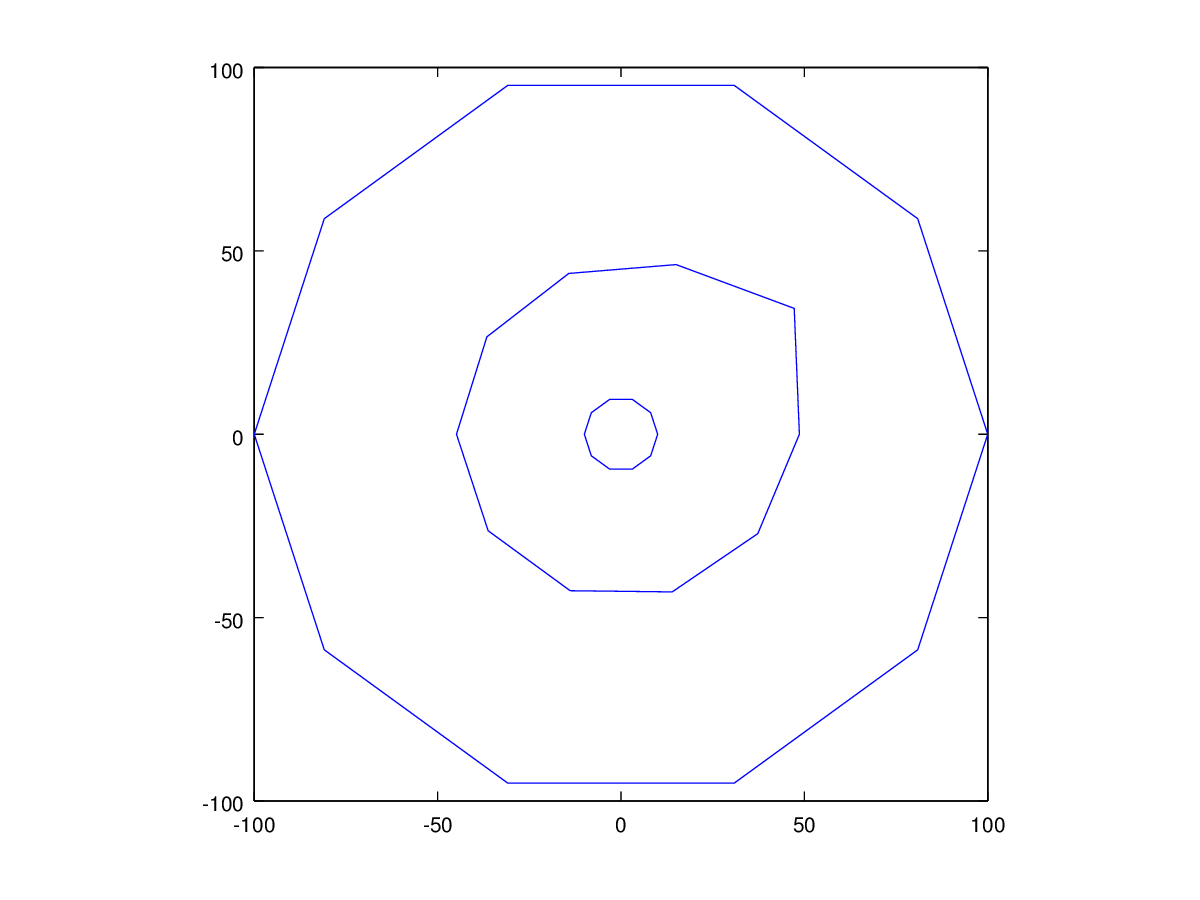
\includegraphics[width=1\textwidth]{imgs/comp_angulos/comp_angs_iso3.png} 
  \caption{}
  \label{fig:comp_angs_iso3}
\end{minipage}%
\hspace{0.03\textwidth}
\begin{minipage}{0.30\textwidth}   
  \centering
    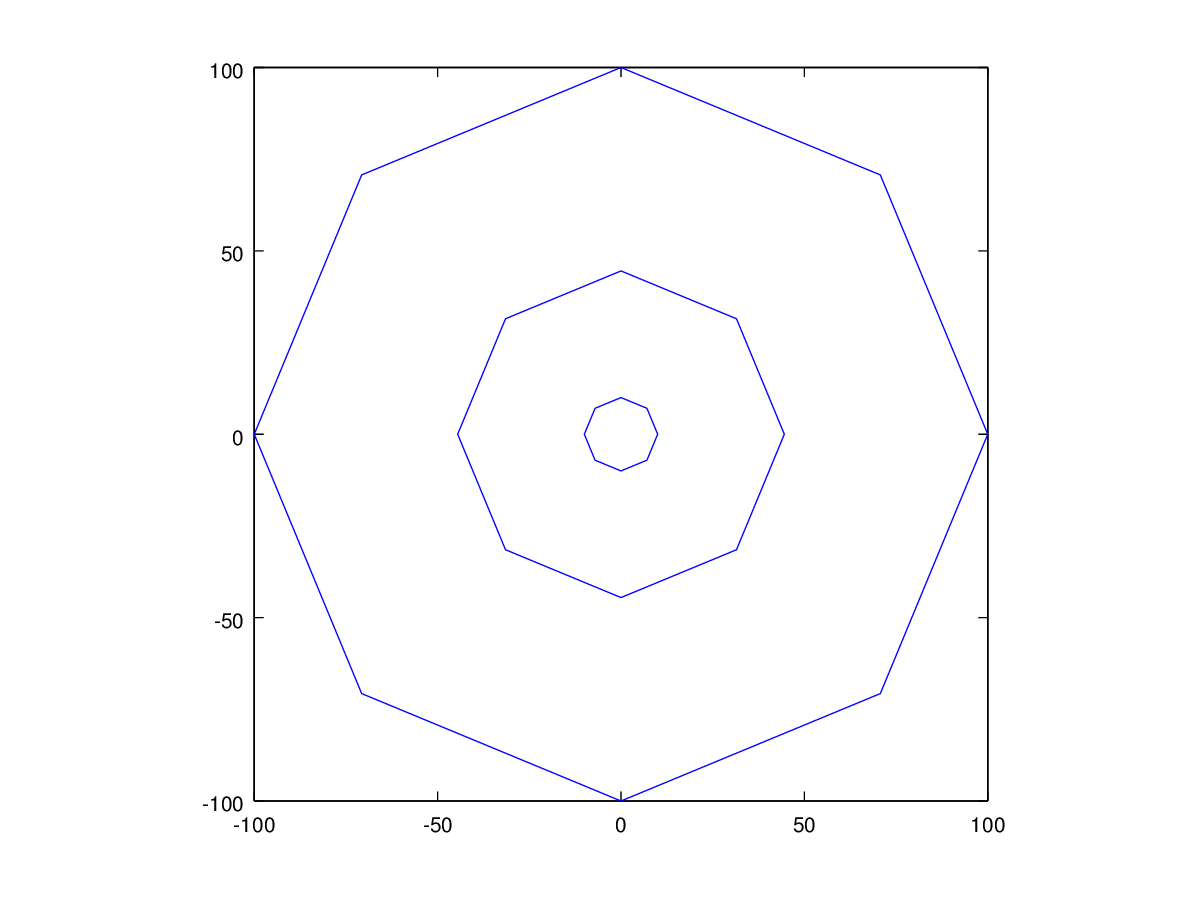
\includegraphics[width=1\textwidth]{imgs/comp_angulos/comp_angs_iso4.png} 
  \caption{}
  \label{fig:comp_angs_iso4}
\end{minipage}
\end{figure}

En las Figuras \ref{fig:comp_angs_temp0} y \ref{fig:comp_angs_iso0}, con 30 ángulos, se puede detectar a la perfección la existencia y ubicación de un pico en la isoterma. Luego, en las Figuras \ref{fig:comp_angs_temp3} y \ref{fig:comp_angs_iso3}, con 10 ángulos si bien se detecta un pico, la forma que se muestra está muy alejada de la real. Nótese por ejemplo que la dirección en la que se encuentra el pico no es la misma que la anterior, además de que el tamaño es distinto. Esto podría causar falsas alarmas o la ausencia de las mismas.
Finalmente, en las Figuras \ref{fig:comp_angs_temp4} y \ref{fig:comp_angs_iso4}, en la que se discretizó con 8 ángulos se puede observar como el pico desaparece fallando dramáticamente la predicción en la forma de la isoterma. 

Para más detalles de la evolución de la isoterma y las temperaturas calculadas en el sistema se recomienda recurrir al link de la sección 2 del apéndice (\ref{sec:links}), en la animación ``comp\_angs\_iso'' se podrá notar con mayor claridad lo nombrado previamente, la isoterma irá marcando el pico con mayor precisión a medida que se utilicen mas ángulos, en los casos en que la cantidad de ángulos sea insuficiente el pico y las temperaturas en esa zona estarán muy distorsionadas, esto se puede observar claramente en ``comp\_angs\_temp'', donde las temperaturas en la zona del pico se calculan de forma imprecisa debido a la utilización de una cantidad de ángulos muy pobre.


\subsubsection{Granularidad de los radios}
Al estudiar las posibilidades en la cantidad de radios a utilizar creemos que observaremos como a mayor granularidad mejora la posición de la isoterma, convergiendo a la posición real. A diferencia de los ángulos, con los radios los picos serán detectados sin tomar demasiadas precauciones pero para asegurar que el tamaño de los picos, y de la isoterma en general, sean predichos de forma confiable se recomendará utilizar una cantidad de radios adecuadamente alta según la necesidad que se tenga.


Para verificar un poco esto experimentamos con muchas instancias de prueba, y llegamos a dos instancias que nos parecieron superadoras, ya que representan la idea principal que queremos dar del comportamiento del sistema cuando se varía la granularidad de los radios.

La primera forma una isoterma con forma de óvalo debido a un aumento en la temperatura externa en dos zonas opuestas. La segunda es un círculo perfecto producido por una temperatura constante a lo largo de todo el interior y exterior del horno. En ambos casos veremos como la figura va cambiando su tamaño al tender a la isoterma real.

En la instancia 1 empezamos con 10 radios y fuimos aumentando de a 10, mientras que en la instancia 2 empezamos con 5 y fuimos aumentando de a 5. Ponemos solo algunos pasos significativos de todo ese camino. Para ver todos los pasos (animados), se puede visitar el link del apéndice, \ref{sec:links}.

\subsubsection*{Instancia 1}


\begin{figure}[H]
\centering
\begin{minipage}{0.30\textwidth}
  \centering
    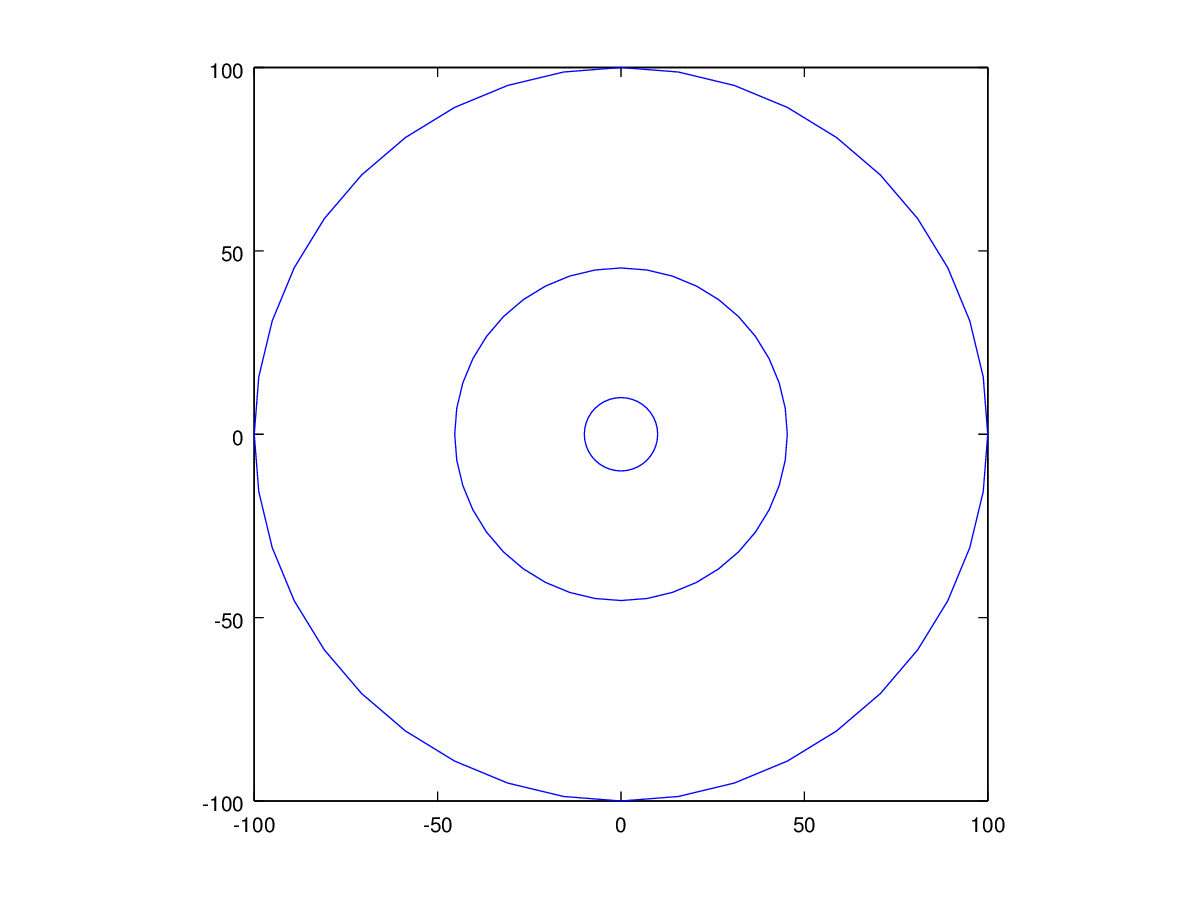
\includegraphics[width=1\textwidth]{imgs/comp_rads_malo/comp_rads_iso5.png}
	\caption{60 radios}  
  \label{fig:Radios4}
\end{minipage}%
\hspace{0.03\textwidth}
\begin{minipage}{0.30\textwidth}   
  \centering
    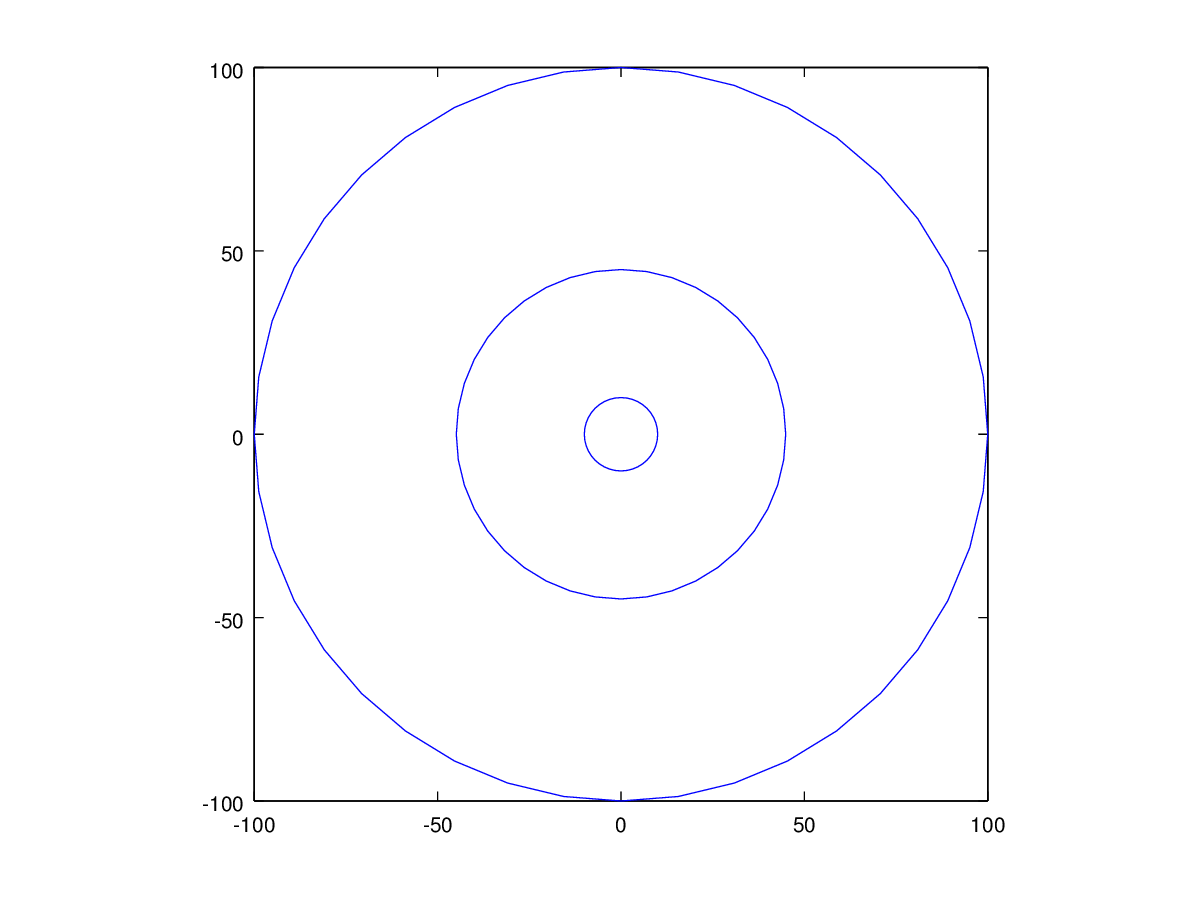
\includegraphics[width=1\textwidth]{imgs/comp_rads_malo/comp_rads_iso3.png} 
	\caption{40 radios} 
  \label{fig:Radios5}
\end{minipage}
\hspace{0.03\textwidth}
\begin{minipage}{0.30\textwidth}   
  \centering
    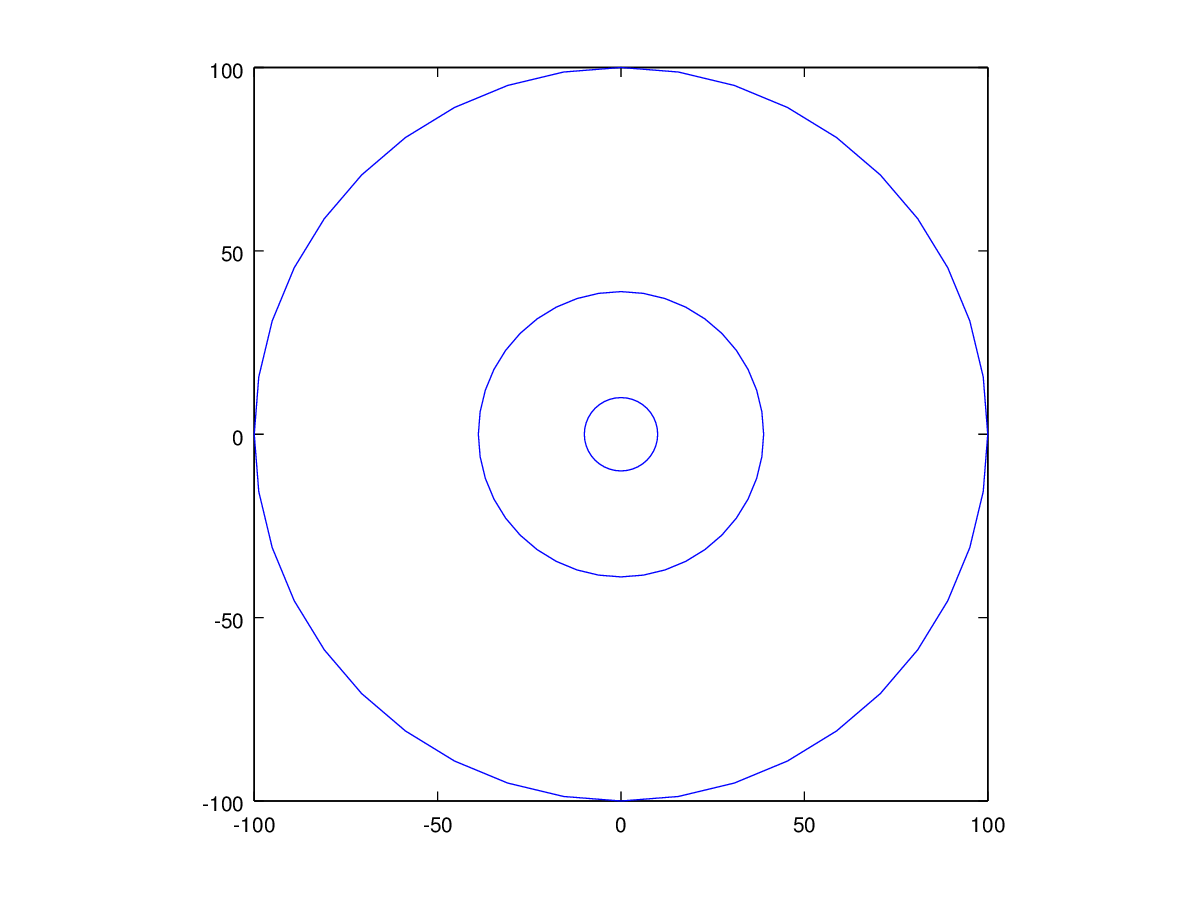
\includegraphics[width=1\textwidth]{imgs/comp_rads_malo/comp_rads_iso0.png} 
	\caption{10 radios} 
  \label{fig:Radios6}
\end{minipage}
\end{figure}

Sucede lo mismo que en en el experimento anterior, al tomar una cantidad relativamente alta de radios se logra un error muy pequeño del tamaño de la isoterma, en este caso se utilizaron 60. La diferencia entre utilizar 40, 50 y 60 radios no fue muy grande, al menos para nuestros estandáres, por lo cual se podrían utilizar simplemente 40 consiguiendo un buena relación entre tiempo de cálculo y aproximación al tamaño de la isoterma.

Para apreciar mejor esto pueden acceder al link de la segunda sección del apéndice (\ref{sec:links}) y ver las animaciones ``comp\_rads\_iso'' y ``comp\_rads\_iso''.




\subsubsection*{Instancia 2}

\begin{figure}[H]
\centering
\begin{minipage}{0.30\textwidth}
  \centering
    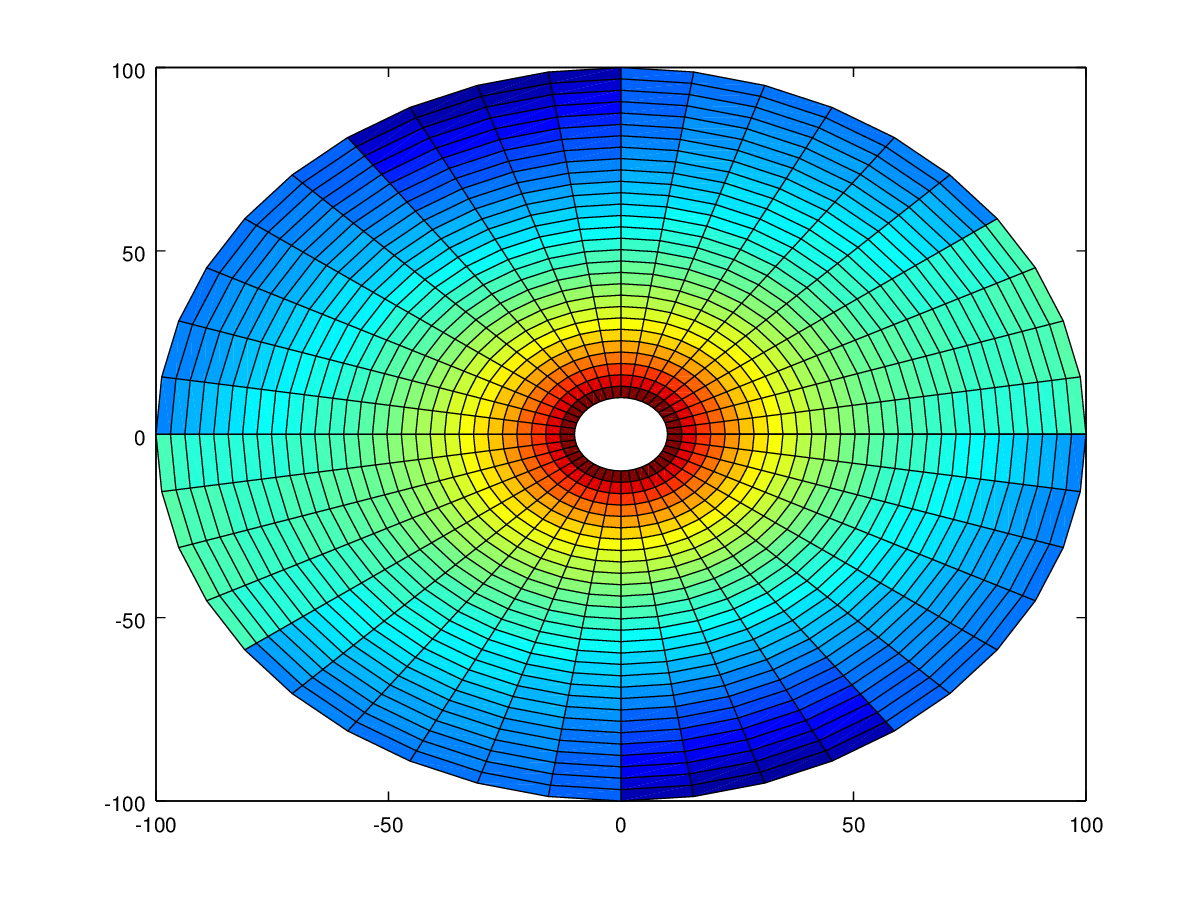
\includegraphics[width=1\textwidth]{imgs/comp_rads_bueno/comp_radss_temp5.png}
  \caption{}
  \label{fig:Radios_1}
\end{minipage}%
\hspace{0.03\textwidth}
\begin{minipage}{0.30\textwidth}   
  \centering
    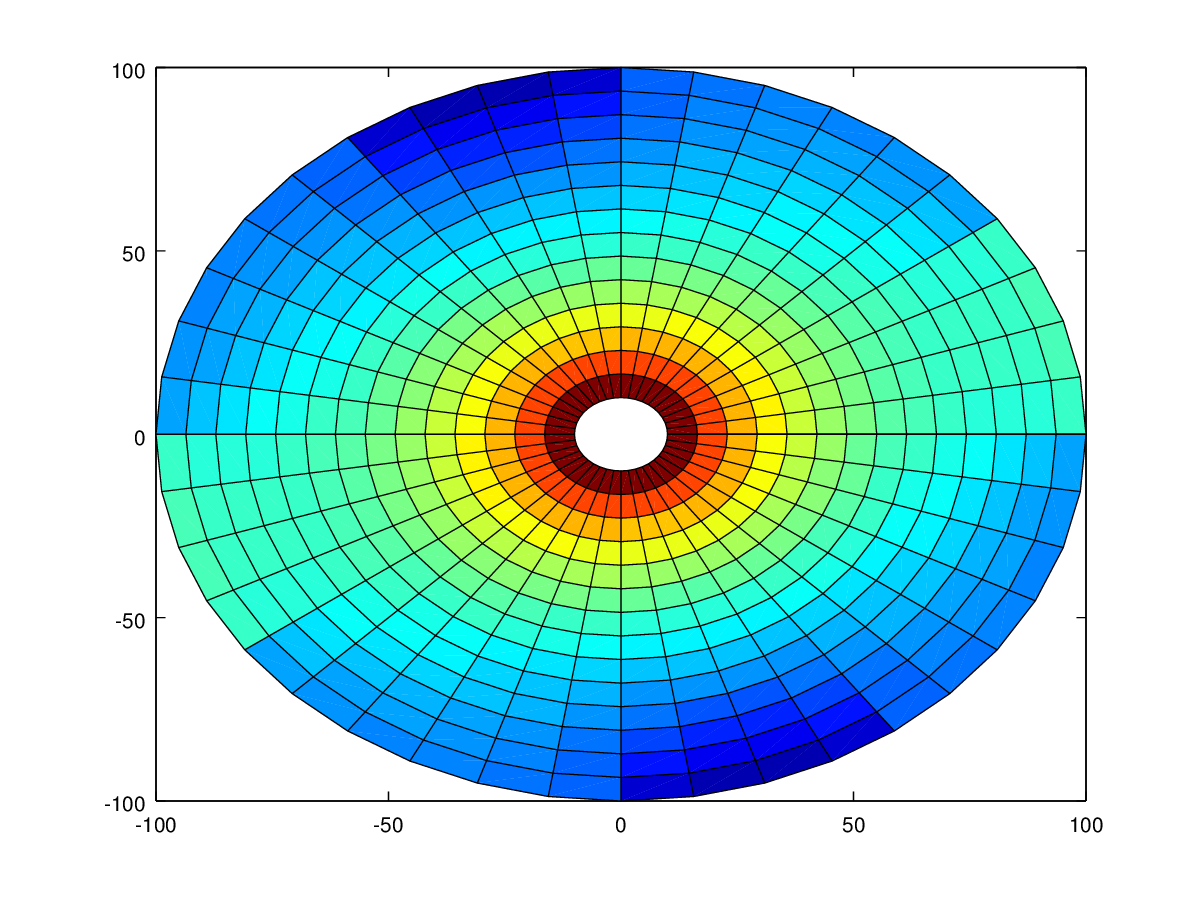
\includegraphics[width=1\textwidth]{imgs/comp_rads_bueno/comp_radss_temp2.png} 
    \caption{} 
  \label{fig:Radios_2}
\end{minipage}
\hspace{0.03\textwidth}
\begin{minipage}{0.30\textwidth}   
  \centering
    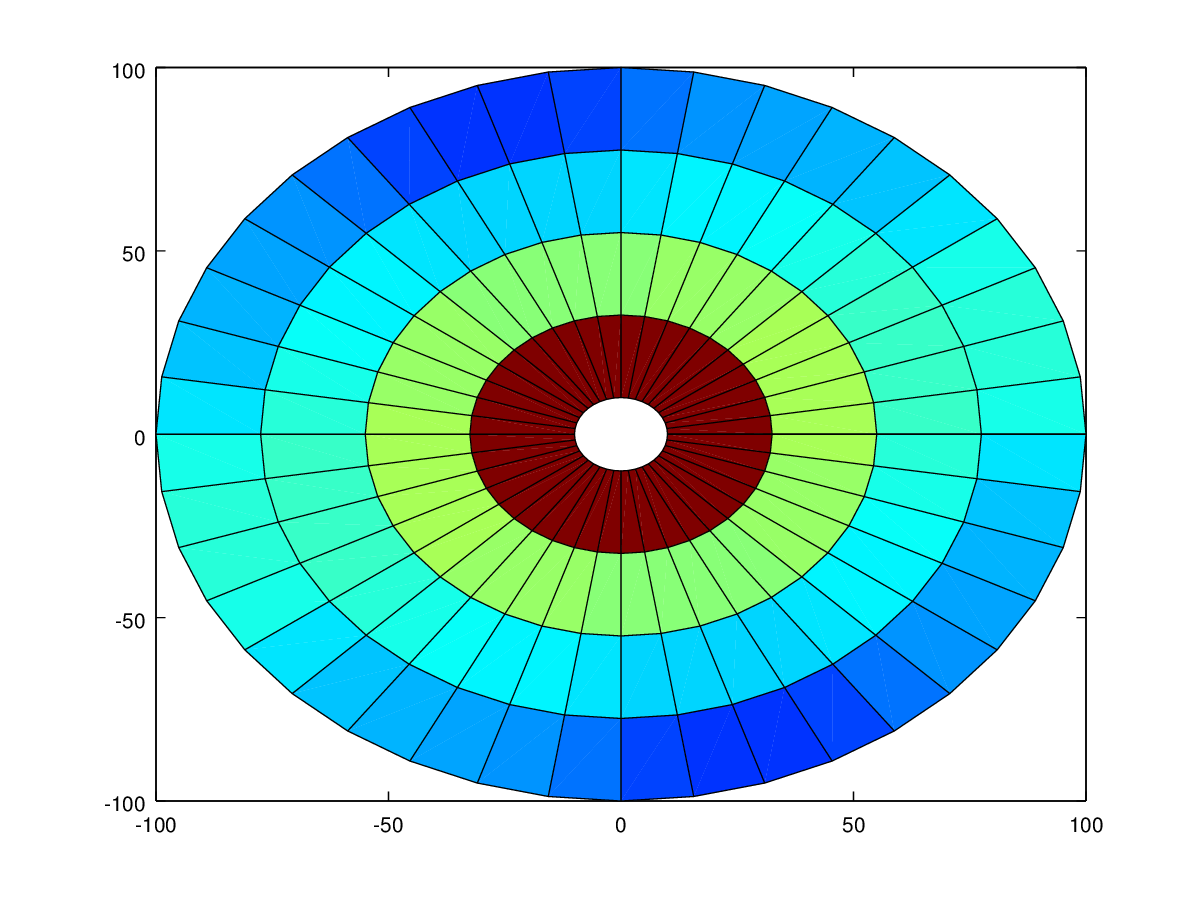
\includegraphics[width=1\textwidth]{imgs/comp_rads_bueno/comp_radss_temp0.png} 
    \caption{} 
  \label{fig:Radios_3}
\end{minipage}
\end{figure}

\begin{figure}[H]
\centering
\begin{minipage}{0.30\textwidth}
  \centering
    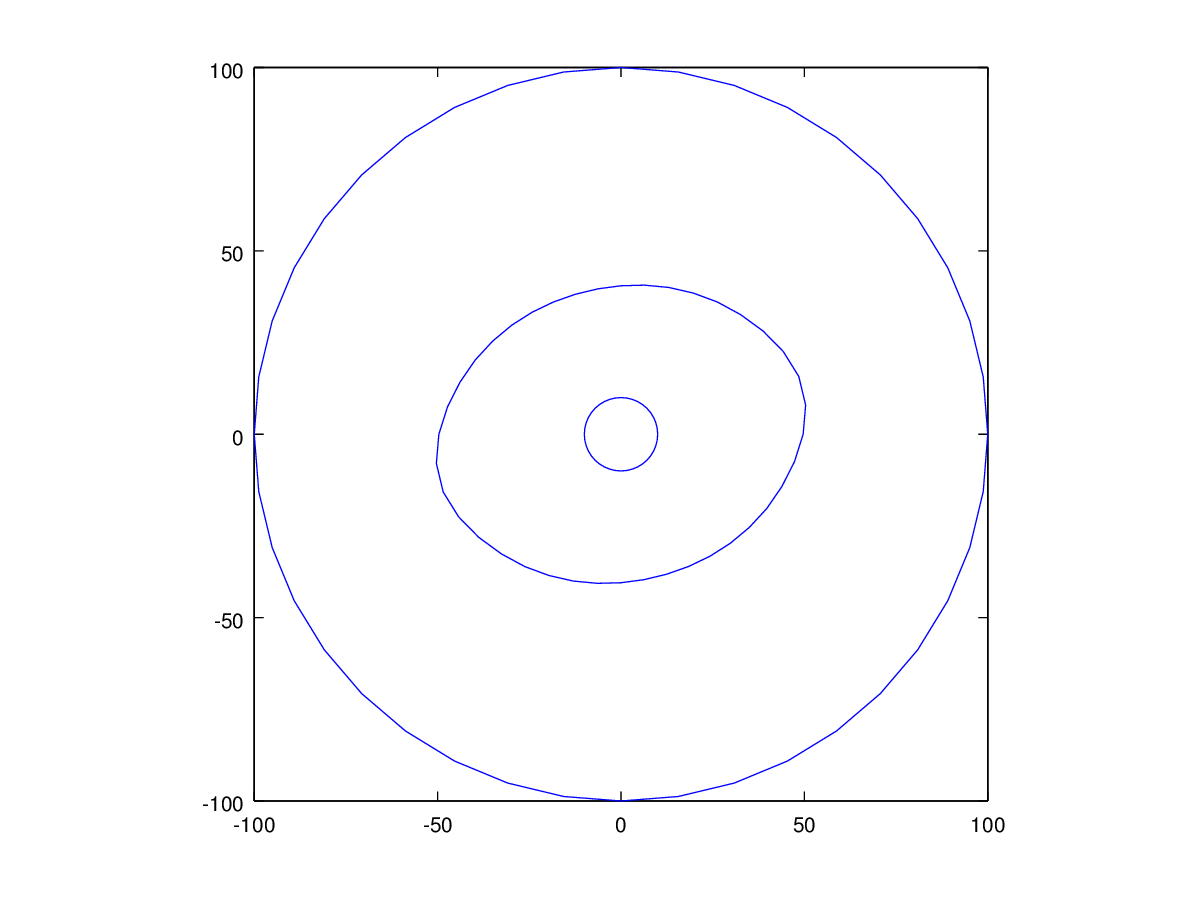
\includegraphics[width=1\textwidth]{imgs/comp_rads_bueno/comp_radss_iso5.png}
  \caption{}
  \label{fig:Radios1}
\end{minipage}%
\hspace{0.03\textwidth}
\begin{minipage}{0.30\textwidth}   
  \centering
    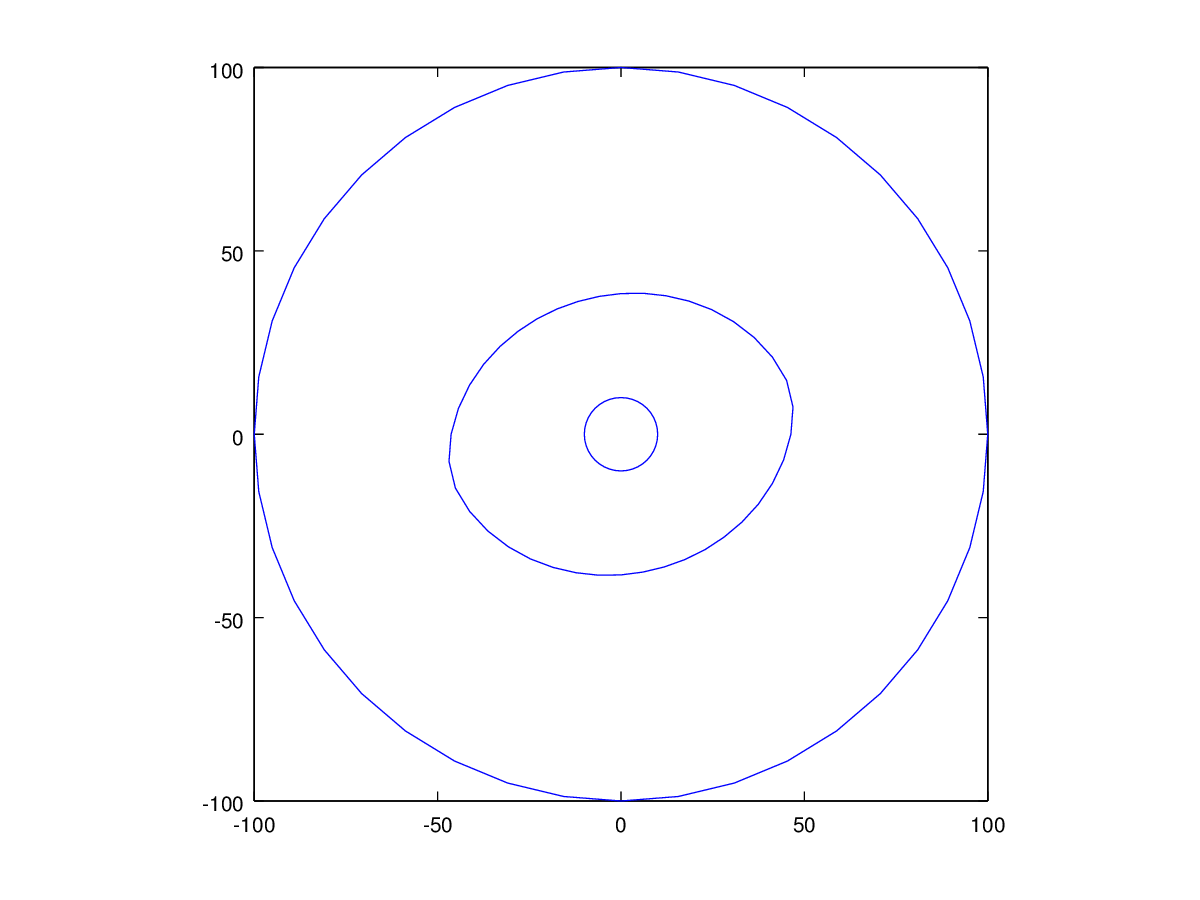
\includegraphics[width=1\textwidth]{imgs/comp_rads_bueno/comp_radss_iso2.png} 
    \caption{} 
  \label{fig:Radios2}
\end{minipage}%
\hspace{0.03\textwidth}
\begin{minipage}{0.30\textwidth}   
  \centering
    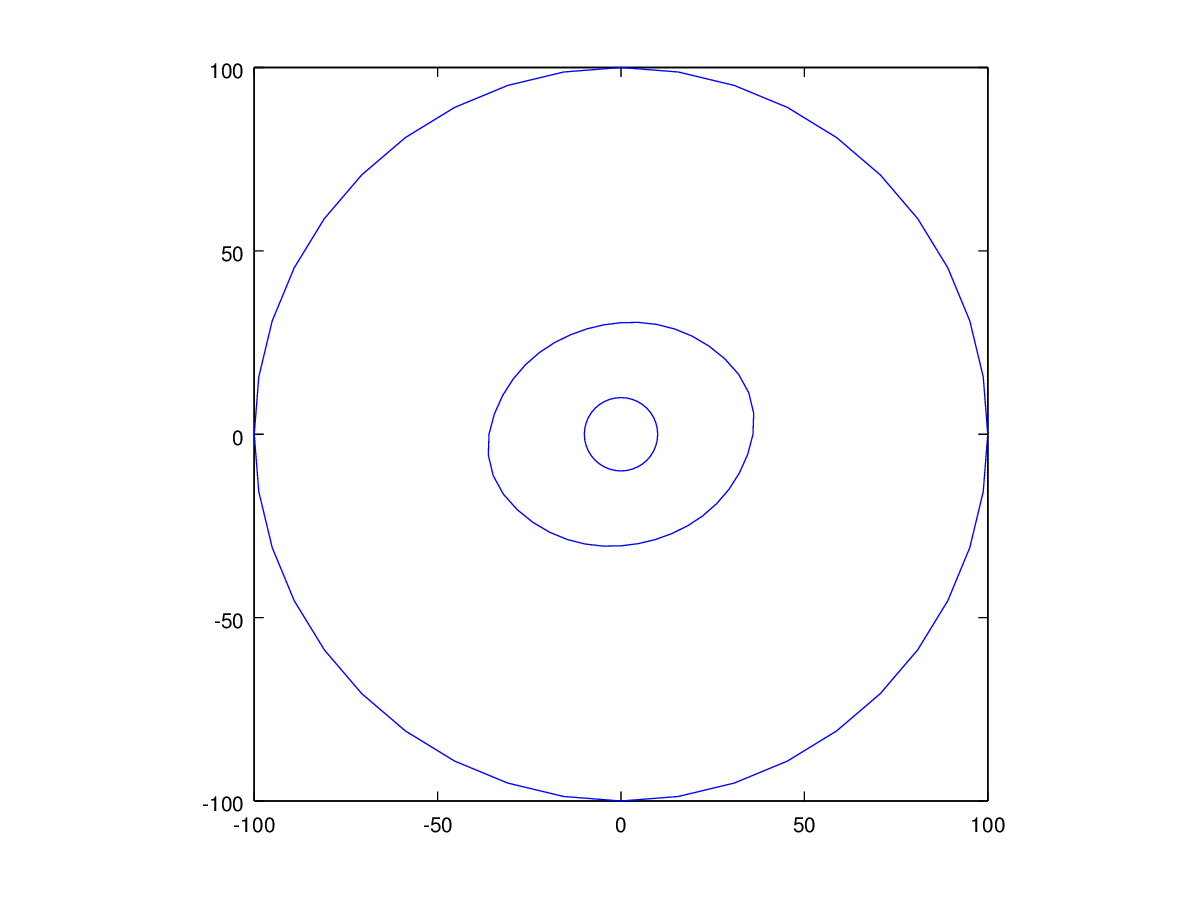
\includegraphics[width=1\textwidth]{imgs/comp_rads_bueno/comp_radss_iso0.png} 
    \caption{} 
  \label{fig:Radios3}
\end{minipage}
\end{figure}

Se puede observar como, a pesar de tener el mismo conjunto de temperaturas exteriores e interiores, y la misma discretización con respecto a los ángulos, hay una gran diferencia entre las Figuras \ref{fig:Radios1} y \ref{fig:Radios_1} , con 30 radios, que consigue una aproximación muy buena del tamaño de la isoterma y las Figuras \ref{fig:Radios3} y \ref{fig:Radios_3} que con sus 5 radios consigue una isoterma muy alejada de la real.

Además, se pueden apreciar los valores intermedios en las Figuras \ref{fig:Radios2} y \ref{fig:Radios_2} (en las que se usan 15 radios) para ver como evolucionan las soluciones frente a estos cambios.

Para apreciar mejor esto pueden acceder al link de la segunda sección del apéndice (\ref{sec:links}) y ver las animaciones ``comp\_rads\_iso2'' y ``comp\_rads\_temp2''.









